% !TeX root = ../../thesis.tex

\subsection{\tcp{}}
Where the previous algorithms both attempted to execute as few tests as possible, it might sometimes be desired or even required that all tests pass. In this case, the previous ideas can be used as well. In \tcp{}, we want to find a permutation of the sequence of all tests instead of eliminating certain tests. The order of the permutation is chosen specifically to achieve a given goal as soon as possible, allowing for early termination of the test suite upon failure \cite{10.1002/stv.430}. Some examples of goals include covering as many lines of code as fast as possible, or early execution of tests with a high probability of failure. A formal definition of this algorithm is provided in \autoref{def:tcp}.

\begin{definition}[\tcp{}]
\label{def:tcp}
\mbox{}\\Given:
\begin{itemize}
	\item $T$ the test suite
	\item $PT$ the set of permutations of $T$
	\item $f: PT \mapsto \mathbb{R}$ a function from a subset to a real number, this function is used to compare sequences of tests to find the optimal permutation.
\end{itemize}

\noindent \tcp{} finds a permutation $T' \in PT$ such that $\forall T'' \in PT : f(T') \ge f(T'') \Rightarrow (T'' \ne T')$ 
\end{definition}

\begin{figure}[htbp!]
	\centering
	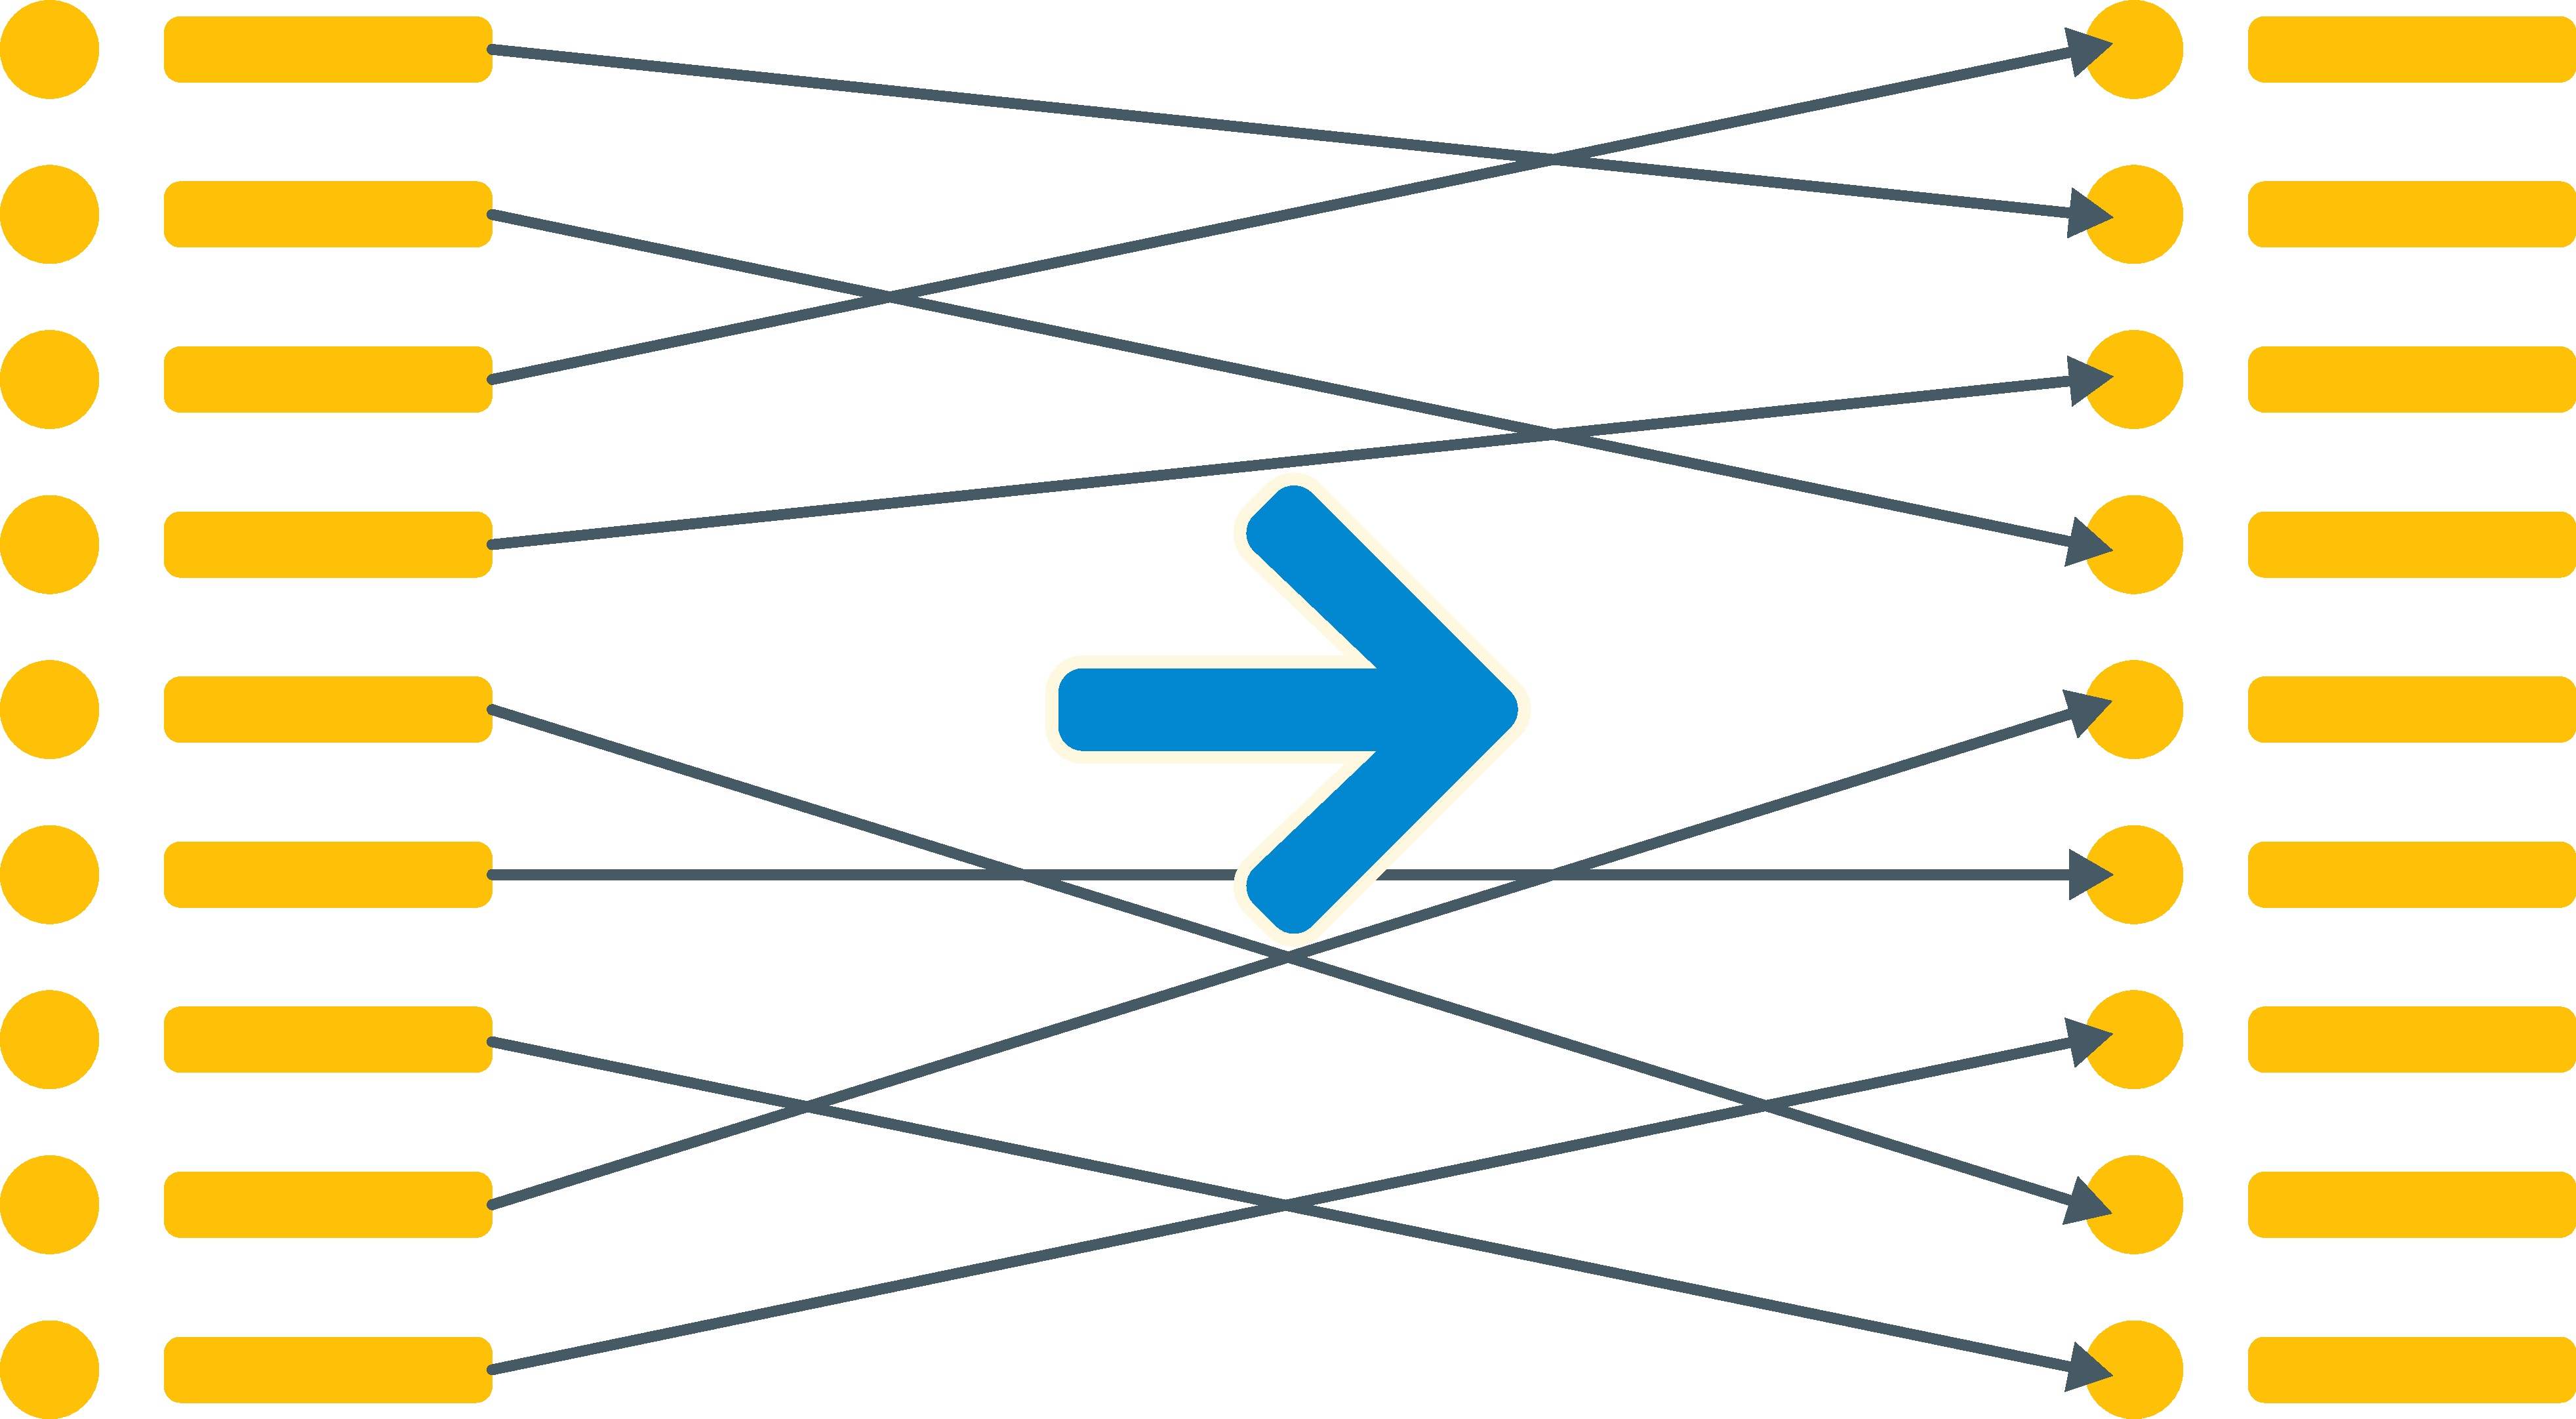
\includegraphics[width=0.6\textwidth]{assets/approach-tcp.pdf}
	\caption{\tcp{}}
	\label{fig:tcp}
\end{figure}